
\chapter{Machine learning}
Machine learning is programming computers to optimize a performance
criterion using example data or past experience. In this chapter we present machine learning applications to challenges posed by big data. In Section \ref{BigD}, we give a brief definition of big data  and the challenges currently faced in radio astronomy. In Section \ref{Intro} we give a brief introduction and examples of machine learning,  and in Section \ref{Process}, \ref{comp} we  present the process of machine learning and model complexity.
\section{Big data}
\label{BigD}
\begin{figure}[H]
  \centering
    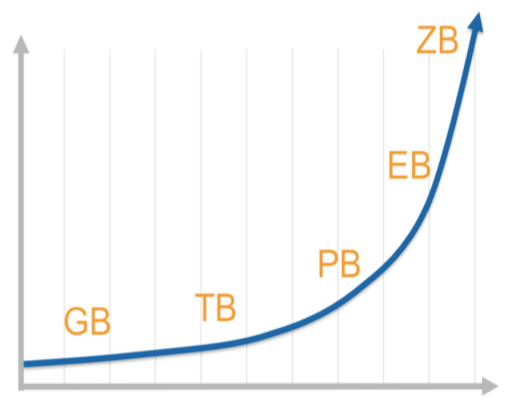
\includegraphics[width=0.5\textwidth]{images/Expgrowth.png}
    \caption{The exponential growth of data from gigabytes to zettabytes [Amazon].}
  \label{datagrowth.png}
\end{figure}

In the past few decades, computing power has been rising exponentially, 
and as a related consequence, enormous quantities and complexity of the observed data, primarily in digital form. Such data are referred to as $\textit{big data}$ and traditional data-processing tools are inadequate to deal with them. In addition to the natural world, big data are now creating a digital world, in which extracting new and useful information from the data already taken and stored is becoming a major endeavor in itself \citep{ball2010data}. This action of knowledge discovery in databases is commonly referred to as \textit{data mining} \citep{ball2010data}. In data mining, a large volume
of data is processed to construct a simple model with valuable use, e.g., having high predictive accuracy  \citep{alpaydin2014introduction}.



\section{An Introduction to machine learning}
\label{Intro}

For a computer to solve a problem, one need an algorithm. An algorithm
is a sequence of instructions carried out to transform
the input to output. e.g, one can design an algorithm for
sorting, where the input is a set of unordered letters and the output is an ordered
list from A to Z. For the same task, there may be various algorithms and one may be
interested in finding the most optimum one, requiring the lowest number of
instructions and memory to run. For some tasks, however, one does not have an algorithm, for example to differentiate between legitimate emails and spam emails \citep{alpaydin2014introduction}. Therefore what we lack in knowledge, we make up for in the collected data. One can easily compile thousands of example messages, some of which one knows to be spam and then we get to learn what characterizes a spam email \citep{alpaydin2014introduction}. 

Learning is what gives humans flexibility, the fact that humans can adjust and adapt to new circumstances and learn new
tricks no matter at any age \citep{marsland2015machine}. The important parts of human or animal learning are adapting, remembering and generalising. Being able to recognize old events, and to know which actions are to be taken, and also knowing how to distinguish between different situations is what makes learning useful \citep{marsland2015machine}. 

 Machine learning is not only a database problem, but is also part
of artificial intelligence. For a system to be intelligent, it needs to have the ability to learn and adapt in any changing environment. If the system can learn and
adapt to changes, then it can easily predict future solutions not provided by the system designer \citep{alpaydin2014introduction}. This involves tasks such as  recognition, prediction, diagnosis, robot control,  
planning etc \citep{nilsson1996introduction}.
Machine learning also helps one find solutions to many problems in robotics, speech recognition and vision. Machine learning is is generally based on programming computers to optimize their performance criterion by using example data that consist of various events. A model is defined
up to some parameters, and part of the learning process is to execute a computer program
to find the optimum parameters of the model using the training data that is based on past experience with different events \citep{alpaydin2014introduction}. The model may be descriptive to gain knowledge from data or predictive to make predictions in the
future.
Machine learning uses the theory of statistics in building mathematical
models, because the core task is making inference from different samples \citep{alpaydin2014introduction}.


Given a class of tasks T, an experience E and measure of performance P, a computer program is said to learn from E with respect to T if the measure P at T improves for more observations E provided \citep{michalski2013machine}. 
\subsection{Examples of machine learning}

We are surrounded by machine learning-based technology, such as online shopping, where  search engines learn how to bring us the best results and a list of the most relevant products related to our search, email (spam filters, smart email categorization, etc)  where anti-spam software learns to filter our email messages into spam or not-spam using simple rule filters. A similar approach is used by Gmail to categorize our emails into primary, social, and promotion inboxes, as well as labelling emails as important. 

In a research paper, "The Learning Behind Gmail Priority Inbox" \citep{aberdeen2010learning}, Google outlines its machine learning approach  and notes: " When a user marks messages in a consistent direction, we perform a real-time increment to their threshold." Every time the user marks an email as important, Gmail learns. The researchers tested the effectiveness of Priority Inbox on Google employees and found that those with Priority Inbox "spent 6\% less time reading email overall, and 13\% less time reading unimportant email.",  Facebook  automatically highlights faces and suggests friends to tag when uploading a photo. A similar approach is used on digital cameras to learn how to detect faces. Smartphones today are equipped with a standard feature to convert voice to text; by pressing a button or saying a particular phrase ("OK Google", for example), you can start speaking and your phone converts the audio into text and recognizes voice commands \citep{Techemergence}.  
Machine learning is also widely used in scientific applications such as astronomy and health.


One common feature of all of these applications is that, in contrast to more
traditional uses of computers, in these cases, owing to the complexity of the patterns that need to be detected, a human programmer will find it difficult to provide finely detailed specification of how to tackle such tasks\citep{shalev2014understanding}.  In recent years, the world's technology has become increased consistently, as shown in Figure \ref
{datagrowth.png}, and this escalation has led to the amount of data available for learning increasing dramatically. We therefore provide several reasons why machine learning is important, given the data challenges.
\begin{itemize}

\item Machine learning methods can often be used to extract the important relationships and correlations of hidden information among big data.

\item The amount of information available about certain tasks might be too large and complex for humans to encode, whereas machines can learn this knowledge accurately and be able to capture more of it than humans would \citep{nilsson1996introduction}.
\end{itemize} 

Our focus will be based mainly on tasks that are beyond human capabilities. These are families of tasks that are related to the analysis of complex large datasets such as astronomical data. With more available stored digital data, it becomes obvious that there is meaningful information buried in the data that is complex for humans
to make sense of. Learning to detect meaningful information in large
 datasets is a promising domain in which the combination
of programs that learn with computers that have high processing power  opens up new horizons \citep{shalev2014understanding}.

\subsection{Types of machine learning}

\begin{figure}[H]
  \centering
    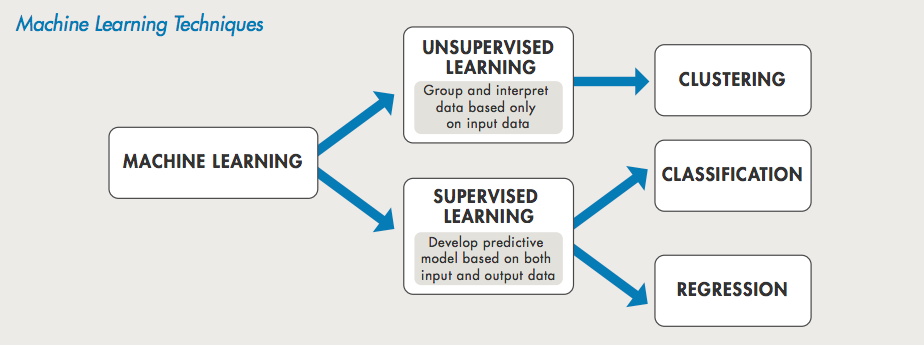
\includegraphics[width=0.7\textwidth]{images/Ml_techs.png}
    \caption{Machine learning techniques include both supervised and unsupervised learning \citep{Machinelearning}.}
  \label{sup-unsup}
\end{figure}

Machine learning algorithms are broadly divided into unsupervised and supervised methods, also known as descriptive and predictive. In supervised learning, the goal is to predict the value of an output measure based on a number of input measures, i.e, finding the relationship between the input and output based on the training dataset. In contrast to supervised learning, unsupervised learning occurs in the sense that the data can speak for themselves
without preconceptions such as expected classes being imposed \citep{ball2010data}. 

\subsubsection{Supervised learning}
The aim of supervised machine learning is to build a model
that makes predictions based on some evidence in the presence. Suppose  one wants to fit a model $\textbf{Y}=f(\textbf{X})+\epsilon$ with errors $\epsilon$ being additive. Supervised learning attempts to learn the function $f$ by examples given through a teacher, given the training set with input and output observations $T=(x_i,y_i ), i=1,\dots N$. The observed input values $x_i$ are fed into a learning algorithm, which produces outputs $\widehat{f}(x_i)$ in response to the given inputs. The learning algorithm has the property that it can modify its input/output relationship $\widehat{f}$ in response to the computed error $y_i- \widehat{f} (x_i)$ between the original and predicted outputs. This process is known as learning by example. Upon completion of the learning process the hope is that the predicted and real outputs will be close enough with an error of approximately zero \citep{friedman2001elements}.

Supervised learning uses regression and classification techniques
to develop predictive models. Depending on the given dataset, variables can be characterized as either qualitative (also known as categorical) or quantitative. Quantitative variables take on numerical values. Examples include a person's height, age, air temperature, wind speed, etc. Whereas, qualitative variables take on input vectors and decide which of N classes
they belong to as shown in Figure \ref{RC}, based on training from exemplars of each class or category. Examples of qualitative variables include a person’s gender (male or female) or whether a person defaults on a debt (yes or no) \citep{aitkin2009statistical}. Qualitative variables are typically represented numerically by codes. The easiest case is when there are only two classes or categories, such as "success"
or "failure", "survived" or "died". These are often represented by a single binary digit or bit as 0 or 1, or else by -1 and 1. For reasons that will become apparent, such numeric codes are sometimes referred to as targets \citep{friedman2001elements}. In machine learning, if the label is numerical, the task is called regression and the learner is also called a fitted regression model, while if the label is categorical, the technique is called classification and the learner is also called a classifier. For both techniques, the training process is conducted on data sets containing label information or examples \citep{zhou2012ensemble}.

\begin{figure}[H]
  \centering
    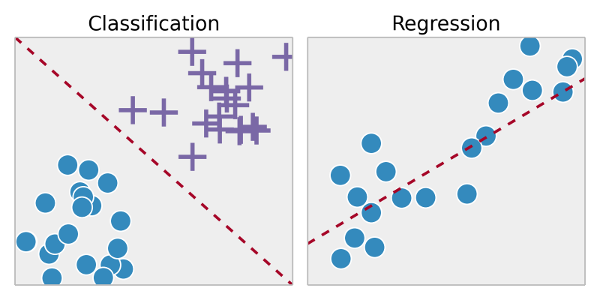
\includegraphics[width=0.7\textwidth]{images/RC.png}
    \caption{Example of classification and regression \citep{rossant2018ipython}.}
  \label{RC}
  
\end{figure}
Classification tasks are mostly known to be discrete, i.e. each example belongs to only one class, and the set of classes covers the whole possible output space; whereas regression tasks are known to be continuous \citep{stephen2009machine}. However there are some overlaps between the algorithms for these tasks. A classification algorithm may predict a continuous value, but the continuous value is in the form of a probability for a class label and a regression algorithm may predict a discrete value, but the discrete value is in the form of an integer quantity. Some algorithms can be used for both classification and regression with small modifications, such as decision trees and artificial neural networks \citep{brownlee2013prepare}.  

\subsubsection{Unsupervised learning}

In contrast to labelled data,  data items without associated labels can often be obtained in great quantities without much effort to be done on it. The unsupervised learning technique aims at making use of the information provided by the unlabelled patterns to generate appropriate models. 

As illustrated in Figure \ref{sup-unsup}, in unsupervised learning one has only a set observations $T=x_1,x_2,\dots, x_N$. In unsupervised learning one is not interested in prediction, because one does not have an associated output response variable $y_1,y_2,\dots, y_N$. Rather the goal in unsupervised learning algorithms is to discover interesting information about the measurements on the training set $T$. One looks for an informative way to visualize the data and interesting patterns among the observations \citep{james2013introduction}. 

\begin{figure}[H]
  \centering
    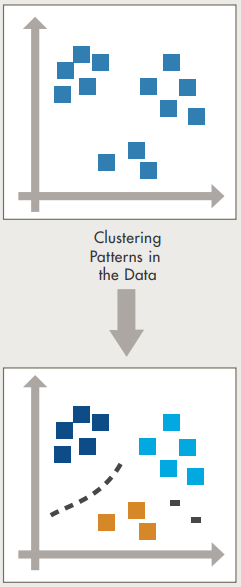
\includegraphics[width=0.35\textwidth]{images/cluster.png}
    \caption{An example of clustering method which reveals hidden patterns in data \citep{Machinelearning}.}
  \label{datagrowth.png}
\end{figure}

Clustering is one of the most commonly used unsupervised methods that divide the data into clusters. The number of clusters must initially be specified with a value K. The algorithm uses a distance
criterion for cluster membership, such as computing the Euclidean distance between the clustered points, and a stopping criterion for iteration\citep{ball2010data}.

\section{Process of machine learning}
\label{Process}
\subsection{Data preparation}
Machine learning algorithms learn from data, therefore it is critical that one feed them the right data for the specific problem one want to solve. In this section we will describe the processing steps required for getting data ready for a machine learning algorithm.

Three steps are commonly used in machine learning to process the data, namely data selection, data preprocessing  and data transformation. Data selection has to do with the selection of the the subsets of all available data that one need to address the question or problem on which we are working. Usually assumptions will be made  about the data and be tested at a later stage. After selecting the data, comes the preprocessing step where one decide how to use the data. Firstly, suitable formatting of the data is considered, which could be .csv file format or Numpy file format. In such cases there may be data instances that are incomplete or do not contain useful information. Such cases, the removal or fixing of such data is required. When generating the training dataset, it is crucial  to also consider the computational cost and memory requirement. Sampling the data by taking a smaller representative sample of the selected data may be much faster for exploring the data space and prototyping solutions before considering the whole dataset. The final step is to transform data using scaling, where the preprocessed data may contain attributes with a mixture of scales for various quantities, which then are scaled to range between 0 and 1. This helps to stop the weights from getting too large unnecessarily \citep{marsland2015machine}. One could also use decompositions, which involve attributes that represent a complex concept that may be more useful to a machine learning method when split into the constituent parts, and  aggregations where attributes can be aggregated into a single attribute that would be more meaningful to the problem being solved \citep{brownlee2013prepare}. The most commonly used scaling methods are referred to as data normalisation, or standardisation \citep{marsland2015machine}.
    
\subsection{Feature engineering}

In machine learning applications, whether classification or regression, observation
dataset that one believes to contain information are taken as inputs and fed
to the model for decision-making. Some of the goals in these learning algorithms are: improving the prediction performance of the model and reducing the model complexity. This could help reduce the estimation error and thus prevent overfitting. If one assumes that the observation dataset $\textbf{X}=\mathbb{R}^d$ \citep{shalev2014understanding}, then the complexity of the model would depend on the number of
input dimensions, $d$, as well as the sample size $N$. 
For reduced memory and computation, one is interested in reducing
the dimensionality of the problem such that one has a new feature space $\mathbb{R}^k$ of dimension $k \ll d $. Decreasing $d$ will also decreases the complexity of the algorithm and increase the learning process speed. The
complexity is often broken into two parts: the complexity of training the algorithm, and the complexity of applying the trained algorithm to new data. Training does not happen very often, and is not usually time-critical. However, we often want a decision about a test point quickly, and there are potentially many test points when an algorithm is in use, so this needs to have low computational cost \citep{marsland2015machine}.

When data can be explained with fewer features, one gets a better idea about the process that underlies the data and this allows knowledge extraction. There are two main methods for reducing dimensionality: feature selection and feature extraction. In feature selection, one is interested in
finding $k$ of the $d$ dimensions that give the most information such that the other $(d - k)$ dimensions are discarded. In feature extraction, one is interested in finding a new set of $k$ dimensions that are combinations of the original $d$ dimensions \citep{alpaydin2014introduction}.
 
During algorithm learning, a feature $x_i\in\mathbb{R}$ becomes relevant to a target concept $t$ (what is being learned) if  a pair of examples A and B in the instance space such that A and B exists differ only in their assignment to  $x_i$ \citep{blum1997selection}. This implies that adjusting the value of $x_i$  will affect the desired output of the learning algorithm. Hence it is important to identify the features that are more important for the problem. This invariably requires prior knowledge of the problem and the data. This process is called feature selection.

In any machine learning, algorithm technique selection is mostly driven by the structure of the dataset and type of problem one wishes to solve (regression or classification). Therefore it is important to have better understanding of the dataset and which features are useful prior to the selection and splitting of the dataset, as described in the previous paragraph. The output of the problem is real number, one therefore categorize the problem as regression. The identified algorithms that are applicable and practical to implement are multi-output regression algorithms to be discussed in more details in the next chapter. 


\section{Tuning model complexity}
\label{comp}
In prediction models, prediction errors can be decomposed into error due to variance and error due to bias of the model. There is a tradeoff between a model's ability to minimize the bias and variance during training \citep{fortmann2012understanding}. 
\subsection{Bias and variance }
Understanding these two types of error can help us diagnose model results and avoid the mistake of over and underfitting. Understanding the bias and variance will help one to improve the data fitting process, resulting in accurate models \citep{fortmann2012understanding}.
Error due to bias is the difference between the average prediction of  models and the true value which one is trying to predict. For example, assuming one has multi-models built from a dataset generated randomly, this will result in the models yielding multi-predictions, hence the bias measures how far off in general these model's predictions are from the true value. Error due to variance is the variability of a model prediction for a given data point \citep{fortmann2012understanding}. 

\begin{figure}[H]
  \centering
    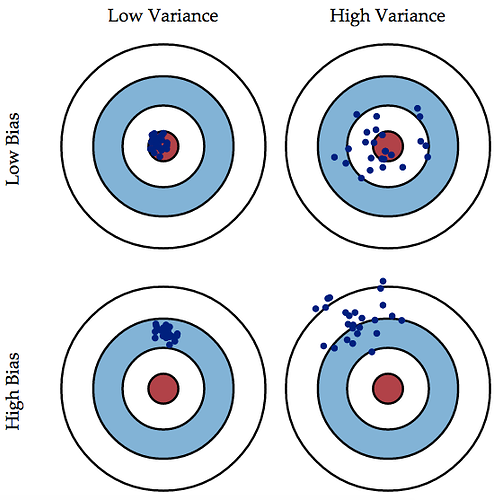
\includegraphics[width=0.48\textwidth]{images/Bias.png}
    \caption{Graphical illustration of bias and variance. The center of each target represents a model that perfectly predicts the true value and as one moves away from the centre, the model gets worse at predicting the true value. Variability in the training dataset due to outliers or non-standard values will also result in poor prediction \citep{fortmann2012understanding}.}
  \label{RC}
 \end{figure}
 
Suppose  one has a training set $\textbf{X}=\{x_1,\dots x_n\}$ and and a function $\textbf{Y}=f(\textbf{X})+\epsilon$ with $\epsilon$ being an error term normally distributed with zero mean and variance $\sigma^2$. One wants to find a function $\widehat{f}(\textbf{X})$  that estimates $f(\textbf{X})$ as well as possible using some learning algorithm technique. In this case, one measures the mean squared prediction error at a point $x$ as :
\begin{align*}
Err(x)&= \mathbb{E}\left[(\textbf{Y}- \widehat{f}(x) ) \right]\\
&= \mathbb{E}\left[ \textbf{Y}^2 +\widehat{f}(\textbf{x})^2 -2\textbf{Y}\widehat{f}(x)\right]\\
&= \mathbb{E}\left[\textbf{Y}^2 \right] + \mathbb{E}\left[\widehat{f}(x)^2 \right]- 2\mathbb{E}\left[\textbf{Y}\widehat{f}(x)\right]
\end{align*}
Since $\text{Var}(\textbf{Y}) = \mathbb{E}\left[\textbf{Y}^2 \right]- \mathbb{E}\left[\textbf{Y}\right]^2$, then we have  $\mathbb{E}\left[\textbf{Y}^2 \right] =\text{Var}(\textbf{Y}) + \mathbb{E}\left[\textbf{Y}\right]^2$, such that
\begin{align*}
Err(x)&= \text{Var}(\textbf{Y}) + \mathbb{E}\left[\textbf{Y}\right]^2 + \text{Var}\left[\widehat{f}(x)\right] + \mathbb{E}\left[\widehat{f}(x) \right]^2- 2f\mathbb{E}\left[\widehat{f}(x) \right]\\
&= \text{Var}(\textbf{Y}) + \text{Var}(\widehat{f}) + (f(x)- \mathbb{E}\left[
\widehat{f}\right]^2)\\
&= \sigma^2 + \text{Var}(\widehat{f})+ \text{Bias}\left[\widehat{f}\right]^2
\end{align*}

where $\sigma^2$ represents the irreducible error \citep{fortmann2012understanding}. 

There are various ways of managing the bias and variance during training, one of them being resampling and bootstrap aggregating. These techniques can be used to reduce the variance in model prediction. In bootstrap aggregating, replicates of the original dataset are created using a random selection with replacement. Each randomly selected data set is then used to construct a new model and the models are combined together into an ensemble. To make a prediction, all the models in the ensemble are averaged \citep{fortmann2012understanding}.

\subsection{Overfitting and underfitting}

\begin{figure}[H]
  \centering
    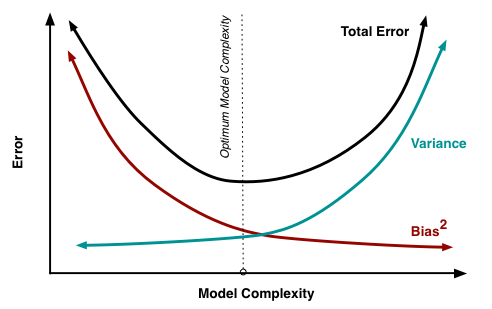
\includegraphics[width=0.7\textwidth]{images/biasvariance.png}
    \caption{The figure is showing the bias and variance contribution to total error. Dealing with bias and variance is about dealing with overfitting and underfitting of the model. The bias is reduced and the variance is increased in relation to the model complexity. As the parameter space of the model increase, the more one experience  complexity whereby the variance increases and becomes the primary concern while bias steadily decreases \citep{fortmann2012understanding}.}  
\end{figure}

Understanding bias and variance is critical for understanding the behaviour of prediction models, but in general what one really cares about is the overall error, not the specific decomposition. The optimum point for any model is the level of complexity at which the increase in bias is equivalent to the reduction in variance as shown in the figure above. If model complexity exceeds this optimum point; we are in effect overfitting our model; while if our complexity falls short of the optimum point, we are underfitting the model \citep{fortmann2012understanding}.

\section{Regression algorithm} 
\label{algo1}
Many different approaches are employed in machine learning regression. These approaches learn the relationship between the input and output by fitting a model directly from the data. The fitting process involves the adjustment and optimization of hyper-parameters to minimize the prediction error. This is usually done in an independent validation and testing dataset. In this study, we consider tree-based approaches: Decision tree, random forest, extremely randomized tree and the neighbourhood search approach: (K-nearest neighbor) to tackle our problem. Firstly, we formulate our regression estimation problem as follows. Suppose we have a feature matrix 
\begin{align*}
\textbf{X}_{t}=\begin{bmatrix}
    x_{11} & x_{12} & x_{13} & \dots  & x_{1n} \\
    x_{21} & x_{22} & x_{23} & \dots  & x_{2n} \\
    \vdots & \vdots & \vdots & \ddots & \vdots \\
    x_{d1} & x_{d2} & x_{d3} & \dots  & x_{dn}
\end{bmatrix}=(x_{i,j}) \in  \mathbb{R}^{d \times n}\;, i\in \left\{1,2,\dots, d\right\}, j \in \left\{1,2,\dots,n\right\}
\end{align*}
where each column represents a vector of length d containing unique features, 
\begin{align*}
\textbf{x}_j=\begin{bmatrix}
    x_{1,j}  \\
    x_{2,j} \\
    \vdots \\
    x_{d,j} 
\end{bmatrix},
\end{align*}
with each row a vector of length n, containing the n variable measurements for the ith observation, i.e 
\begin{align*}
\textbf{x}_i=\begin{bmatrix}
    x_{i,1}  \\
    x_{i,2} \\
    \vdots \\
    x_{i,n} 
\end{bmatrix},
\end{align*}

and we also have a matrix of complex target variables to learn and predict on,
\begin{align*}
\textbf{Y}_{t}=\begin{bmatrix}
    y_{11} & y_{12} & y_{13} & \dots  & y_{1m} \\
    x_{21} & y_{22} & y_{23} & \dots  & y_{2m} \\
    \vdots & \vdots & \vdots & \ddots & \vdots \\
    y_{d1} & y_{d2} & y_{d3} & \dots  & y_{dm}
\end{bmatrix}=(y_{k,l}) \in  \mathbb{C}^{d \times m},  k\in \left\{1,2,\dots, d\right\}, l \in \left\{1,2,\dots,m\right\}
\end{align*}
where each column represents a vector of length d, containing unique target variables as a function of time $t$
\begin{align*}
\textbf{y}_{l}=\begin{bmatrix}
    y_{1,l}  \\
    y_{2,l} \\
    \vdots \\
    y_{d,l} 
\end{bmatrix},
\end{align*} 
with each row a vector of length m, containing the m variable measurements for the $kth$ observation, that is 
\begin{align*}
\textbf{y}_k=\begin{bmatrix}
    y_{k,1}  \\
    y_{k,2} \\
    \vdots \\
    y_{k,m} 
\end{bmatrix},
\end{align*}
 
The problem is to construct a learning machine, $M:\textbf{X}_{t} \rightarrow \textbf{Y}_{t}$, which when given a validation set of sensor examples, $\textbf{X}^*_{t}$, minimises some measure of discrepancy between its prediction $M(\textbf{X}^*_{t})\approx\widehat{\textbf{Y}}_{t}$, and the value of $\textbf{Y}_{t}$, where M represents the predictor. We measure the discrepancy using four commonly used statistical measures in regression \citep{borchani2015survey}: coefficient of determination, explained variance, mean squared error (MSE) and mean absolute error (MAE). The coefficient of determination is given by:

\begin{equation}
R^2\left[\textbf{Y}_{t},\widehat{\textbf{Y}}_{t}\right]=1-\frac{\sum_{k} \left[(\textbf{Y}_{t})_{k}-(\widehat{\textbf{Y}}_{t})_{k}\right]^2}{\sum_{k}\left[(\textbf{Y}_{t})_{k}-\overline{\textbf{Y}_{t}}\right]^2}, 0 \leq R^2 \leq 1,
\label{R2score}
\end{equation}
which simply measures how well the future observations are to be predicted by M, with the best score being 1 for the best performing predictor 
where,  \begin{equation}
\overline{\textbf{Y}_{t}}=\frac{1}{d_{\mathrm{samples}}} \sum_{k} (\textbf{Y}_{t})_{k},
\end{equation} 

is the mean value of $\textbf{Y}_{t}$ draw from d samples,  
 $\sum_{k}\left[(\textbf{Y}_{t})_{k}-\overline{\textbf{Y}_{t}}\right]^2$ is the total sum of squares which measures the total variance in the predictor and $\sum_{k} \left[(\textbf{Y}_{t})_{k}-(\widehat{\textbf{Y}}_{t})_{k}\right]^2$ the residual sum of squares (deviations predicted from actual values of data), which measures the discrepancy between $\textbf{Y}_{t}$ and $\widehat{\textbf{Y}}_{t}$ \citep{james2013introduction}.

The explained variance
\begin{equation}
V=\frac{\text{Var}\left[\textbf{Y}_{t}-\widehat{\textbf{Y}}_{t} \right]}{\text{Var}\left[\textbf{Y}_{t}\right]}, 0 \leq V \leq 1, 
\label{ExV}
\end{equation}  

measures the proportion to which the predictor accounts for the variation of the observed data $\textbf{Y}_{t}$ \citep{bellinger2016fundamental}. The best possible score is considered to be 1. where 

\begin{align*}
\text{Var}\left[\textbf{Y}_{t}\right]&=\mathbb{E}\left[(\textbf{Y}_{t}-\mu)^2\right],\; \mu=\mathbb{E}\left[\textbf{Y}_{t}\right]\\
&=\mathbb{E}\left[\textbf{Y}_{t}^2-2\textbf{Y}_{t} \mu +\mu^2\right]\\
&=\mathbb{E}(\textbf{Y}_{t}^2)- 2\mathbb{E}(\textbf{Y}_{t} \mu) + \mu^2\\
&=\mathbb{E}(\textbf{Y}_{t}^2)-2 \mu^2 + \mu^2\\
&=\mathbb{E}(\textbf{Y}_{t}^2)-\mu^2,
\end{align*}
\citep{fortmann2012understanding}

MSE and MAE, which measure the average of the squared and absolute of the errors between the the observed values $\textbf{Y}_{t}$ and the predicted $\widehat{\textbf{Y}}_{t}$. For accurate prediction of the predictor, the value of MSE and MAE should converge to zero \citep{james2013introduction}. 

\begin{align}
\text{MSE}\left(\textbf{Y}_{t},\widehat{\textbf{Y}}_{t} \right)=\frac{1}{d_\mathrm{samples}} \sum_{k} (\textbf{Y}_{t}-\widehat{\textbf{Y}}_{t})^2_{k}
\label{MSE}
\end{align}

\begin{align}
\text{MAE}\left(\textbf{Y}_{t},\widehat{\textbf{Y}}_{t} \right)=\frac{1}{d_\mathrm{samples}} \sum_{k} \left|\textbf{Y}_{t}-\widehat{\textbf{Y}}_{t}\right|_{k}
\label{MAE}
\end{align}.

The aim of this regression exercise is to predict multiple target variables $\widehat{\textbf{Y}}_{t}$  hence it is referred to as multi-output regression. The learned model will then be used to  predict multi-output values $\widehat{\textbf{Y}}_{t+1}$  of all target variables of the new incoming unlabelled instances $\textbf{X}_{t+1}$. It has been proven that multi-output regression methods provide means to model the multi-output datasets effectively and produce better predictive results. This method does not only consider  the underlying relationships
between the features and the corresponding targets but also the relationships between
the targets themselves, thereby producing simpler models with better computational efficiency \citep{borchani2015survey}. \citep{borchani2015survey} discuss several applications of multi-output regression including the challenges such as missing data, i.e., when some features or target variables are not observed.

\subsection{Decision tree}
\label{Dt}
Decision tree algorithms are popular methods for machine learning tasks such as classification and regression. These algorithms make it easy to handle categorical features, interpret, extend to the multi-output for regression settings and multiclass for classification setting. They can handle datasets that may have errors or missing values and are able to capture non-linearities and feature interactions \citep{DT}, hence they are widely used. One of the biggest advantages of using decision trees is the ease with which one can see what features or variables contribute to the classification or regression and their relative importance based on their location in the tree.

For a response variable that
has classes, the tree algorithm (classification) organizes the dataset into groups by the response based on the similarities of the data, and when the response variable is numeric or continuous, the tree algorithm (regression) uses the data to predict the outcome by fitting the regression model in each of the independent variables \citep{morgan2014classification}.

Decision trees are a simple but powerful form of multi-variable analysis. In effect, they  perform a recursive binary partitioning of the feature space. The process of the parent node splitting into exactly two child nodes is refereed to as binary\citep{moisen2008classification}, and it is said to be recursive if each child node wil, in turn, become a parent node, unless it is a terminal node, as illustrated in Figure \ref{images/DecisionTree}, where the split occurs at the decision node.  

Decision trees are built by growing a tree upside down, starting from the root node. The data sample passes down the tree through a series of splits, or nodes, at which a decision is made on the direction in which to proceed, either the left or right sub-tree, based on a sequence of questions about the features \citep{musicant2007supervised}. The next split or decision made depends on the answers to previous questions. Eventually, a terminal node is reached and the prediction is made.  

 \begin{figure}[H]
  \centering
    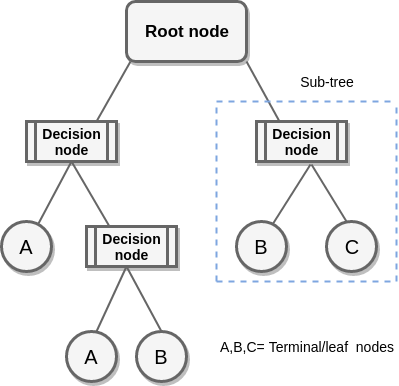
\includegraphics[width=0.6\textwidth]{images/DC.png}
    \caption{An illustration of a decision tree where a recursive partition is shown from the root node where there is an entire data sample to the internal nodes (decision nodes) where splitting occurs to form child nodes, which are either decision nodes or terminal nodes. A terminal node implies that after this split, further splitting of the samples does not provide relevant information in predicting the response variable \citep{moisen2008classification}. }
  \label{images/DecisionTree}
\end{figure}

The binary recursive partitioning can apply to the fitting of both regression and classification trees. Each node in a tree is split based on its impurity, which is a measure of how badly the samples at that node fits the model defined in equation \ref{model}. Therefore, in regression and classification trees, variables and the locations of the split are
chosen to minimize the impurity of the node at that point. However, the selection criteria of splitting each node are different for these two methods. In our case the for the regression scenario, the splitting rules used to minimize the impurity of each node $c$ is the MSE and MAE as defined in equations \ref{MSE} and \ref{MAE} \citep{morgan2014classification}. The sample mean of the response variable (estimated value $\mu_{c}$) that represents the assigned prediction in each terminal node is defined as: 
\begin{align}
\mu_{c}=\frac{1}{N_{c}} \sum_{i\in N_{c}} \textbf{Y}_{i},
\label{model}
\end{align} 
where $N_{c}$ is the number of samples in each node, and $\textbf{X}_{c}$ is the training samples. 
 
These methods not only measure the impurity in each node, but are also used to measure the accuracy of the predictor, as in equations \ref{MSE} and \ref{MAE}. Another commonly used strategy or measure in classification problems which also applies in regression problem, for selecting the best splits, from a set of possible split is to maximize the information gain at each tree node; i.e., the split chosen at each decision node is chosen from the the set $\mathrm{argmax (IG(\textbf{X}_{c},s))}$ where $\mathrm{IG}(\textbf{X}_{c},s)$ is the information gain when a split $s$ is applied to sample data $\textbf{X}_c$. This is the difference between the parent node (decision node) impurity and the weighted sum of the child nodes in equation \ref{IG}. 
 
 \begin{align}
 \mathrm{IG}(\textbf{X}_c,s)&= \mathrm{Impurity}(\textbf{X}_c)-\frac{N_{c(\mathrm{left})}}{N_c}\times \mathrm{Impurity}(\textbf{X}_{c(\mathrm{left})})- \frac{N_{c(\mathrm{right})}}{N_c}\times \mathrm{Impurity} (\textbf{X}_{c(\mathrm{right})}), \label{IG}
 \end{align}
 where $s$ is a split partitioning the training sample $\textbf{X}_c$ of size $N_c$ into two datasets $\textbf{X}_{c(\mathrm{left})}$ and $\textbf{X}_{c(\mathrm{left})}$ each of size $N_{c(\mathrm{left})}$ and $N_{c(\mathrm{right})}$.
If the impurity measure is the MSE, we therefore define the information gain by
 \begin{align}
 \mathrm{IG}(\textbf{X}_c,s)&= \mathrm{Impurity}(\textbf{X}_c)-\frac{N_{c(\mathrm{left})}}{N_c}\times \text{MSE}_{(\mathrm{left})}- \frac{N_{c(\mathrm{right})}}{N_c}\times \text{MSE}_{(\mathrm{right})}.
  \end{align}
If the impurity measure is the MAE, the information gain is defined by   
 \begin{align}
 \mathrm{IG}(\textbf{X}_c,s)&= \mathrm{Impurity}(\textbf{X}_c)-\frac{N_{c(\mathrm{left})}}{N_c}\times \text{MAE}_{(\mathrm{left})}- \frac{N_{c(\mathrm{right})}}{N_c}\times \text{MAE}_{(\mathrm{right})}. 
 \end{align}
 
For multi-output decision trees that predict multiple continuous target attributes at once, the advantage over building a separate
regression tree for each target is that the built tree is usually much smaller than the total size of the individual single-target decision trees for all variables; secondly they  identify easily the dependencies between the different target variables.

The building of the multi-output decision trees follows  the same steps as the standard decision tree in Figure \ref{images/DecisionTree}, starting with all instances in the root node, then iteratively finding the optimal split and partitioning the nodes accordingly until a terminal node is reached, given a certain stopping criterion as shown in Figure \ref{images/DecisionTree}. The only difference  is the redefinition of the impurity measures in equations \ref{MSE} and \ref{MAE} of a node as the sum of the squared error  over a multi-target response. 
\begin{align}
\sum_{k\in d}\frac{1}{N}\left[\sum_{l \in N }\left(\textbf{y}_{k}^{(l)}-\mu^{(l)} \right)^2\right],
\end{align}
where $\mu^{(l)}$ denotes the predicted output for the instance $l$ in each node. Each split is selected to minimize the sum of the squared error such that each terminal leaf of the tree can be characterized by the multivariate mean
of its instances and its defining feature values.

\subsection{Random forest}
Much work has been done in machine learning to improve the predictive ability of regression and classification trees by combining separate tree models into what is often called ensemble.

A random forest is a forest (ensemble) of decision tree predictors such that each tree depends on the values of a random vector sampled independently and with the same distribution for all trees in the forest \citep{breiman2001random}. Figure \ref{random tree} is illustrating how trees are built from randomly sampled data. The random forest algorithm  was introduced by \citep{ho1995random} after having noticed that decision trees were limited in their accuracy especially on large data samples owing to their inability to grow which led to overfitting. The random forest method was found not only to be accurate, but also less susceptible to overfitting.

 \begin{figure}[H]
  \centering
    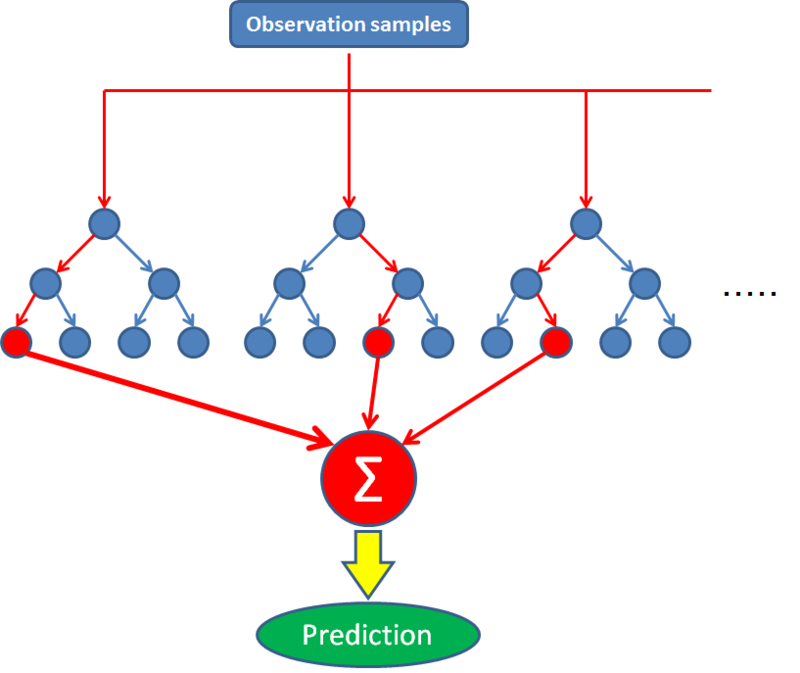
\includegraphics[width=0.6\textwidth]{images/RandomForestTree.png}
    \caption{Random forest regression. [image by Data scientist TJO in Tokyo]}
  \label{random tree}
\end{figure}

In random forest, the randomness is only introduced into the feature selection process, not into the choice of split points on the selected features. During the construction of a component decision tree, at each step
of  the split selection, a random forest first randomly selects a subset of features, and then carries out the split selection procedure for that particular tree within the selected
feature subset. Random forest are considered as an extension of bootstrap aggregating (bagging), where the major difference with bagging is the incorporation of randomized feature selection \citep{zhou2012ensemble}. The operational procedure of bagging is as follows: 

\begin{itemize}
\item Given a  set $\textbf{X}$ of size $\textit{N}$.
\item Generate $\textit{m}$ subsets in vector $\Theta$  of length $\textit{n}$ by randomly selecting data from the set $\textbf{X}$ with replacement \citep{breiman2001random}. 
\item Run $\textit{k}$ number of trees for each of the $\textit{m}$ sets of $\Theta$ to train the data, thereby $\Theta_{\textit{m}}$ sets of trained data  \citep{breiman2001random}.
\item For the remaining $\textit{n}$ samples, trained trees from the previous two steps can be fitted onto the remaining
data set of $\textbf{X}_{\textit{n}}$ to estimate the features of the data  \citep{breiman2001random}.
\end{itemize}

The parameter $\textit{k}$ is the logarithm of the number of features \citep{breiman2001random}. This parameter controls the incorporation of randomness and this results in an increase in the bias. When $\textit{k} =  \text{total\;number\; of\; features}$, then the constructed decision tree will be identical to the traditional deterministic decision tree,  and when $\textit{k}$ = 1, a feature will be selected randomly.

The Random forest performs the prediction of its constructed trees by aggregating all the trees, i.e. (majority voting for classification or averaging for regression) to produce the final output. Suppose the underlying true function we try to learn is $f(\textbf{x})$, and $\textbf{x}$ is sampled according to a distribution p($\textbf{x}$). The output of each decision tree learner can be written as the the true value plus an error item, i.e.,
\begin{align}
h_{i}(\textbf{x})= f(\textbf{x}) + \epsilon_{i} (\textbf{x}), i = 1, \dots,T.
\label{hx}
\end{align}
such that we have the averaging and, 
\begin{align}
H(\textbf{x})= \frac{1}{T}\sum_{i=1}^{T} h_{i}(\textbf{x}). 
\label{averageRF}
\end{align}
\citep{zhou2012ensemble}

Recall in Section \ref{Dt}, that the prediction of  each tree is the sample mean, then from equation \ref{hx} we thus have the MSE of the output prediction $h_i$ as 
\begin{align}
\int (f(\textbf{x})-h_{i}(\textbf{x}))p(\textbf{x})^2d\textbf{x} = \int \epsilon_{i} (\textbf{x})^2 p(\textbf{x})d\textbf{x}.
\end{align}
Similarly, we can derive the MSE of the combined decision tree learner (i.e., the ensemble) as 

\begin{align}
\int \left(f(\textbf{x}) - \frac{1}{T}\sum_{i=1}^{T} h_{i}(\textbf{x}) \right)^2  p(\textbf{x})d\textbf{x} = \int \left( \frac{1}{T}\sum_{i=1}^{T} \epsilon_{i}(\textbf{x})\right)p(\textbf{x})d\textbf{x}
\end{align} 


The two main parameters of a random forest are the number of trees grown and the number of predictors randomly tried at each split. What one calls depth is sometimes found as the maximum node size, and controls the size of the trees that are grown. In the original implementation of random forest, trees are grown to the maximum potential extent so that they reach the lowest possible bias. Then, variance is reduced by growing many trees and averaging them. The main reason is that in random forest, one can only decrease error by reducing the variance, so the bias needs to be as low as possible in the first place. Therefore, in most cases, one does not really need to adjust this parameter (depth or max nodesize). but just has to make sure the default value allows the trees to grow as deeply as possible.

\subsection{K-nearest neighbour}

The K-nearest neighbor algorithm is a well known non-parametric algorithm commonly used for regression and classification problems. K-nearest neighbor is considered to be one of the simplest and yet powerful algorithms that does not make any assumptions about the distribution of the data being evaluated. The learning technique used in K-nearest neigbors is known as the instance-based learning. This technique is based on the memorization of the training dataset and the number of parameters is unbounded and grows with the size of the data. 

The intuition underlying nearest neighbor regression is quite straightforward;
the output predictions are obtained by looking into the memorized examples where the cost of the learning process is 0. The cost is in the computation of the prediction, with the prediction output being the continuous average values (or median) of the values of its K-nearest neighbors. The commonly used measure in K-nearest neighbors is the distance functions , i.e., consider $\mathcal{M}$ the m-dimensional Euclidean space $\mathbb{R}^m$  , a training data set $\textbf{X}=\{\textbf{x}_1,\dots, \textbf{x}_n\} \subset \mathcal{M}$, a query point $q\in \mathcal{M}$, and a distance metric $d:\mathcal{M}^2 \rightarrow \mathbb{R}$. The K-nearest neighbor search is the task of finding  the K closest (w.r.t. $d$ ) points to $q$ from the data set $\textbf{X}$, i.e., we find a set $\textbf{A} \subset \textbf{X}$ for which it holds  that $|\textbf{A}|= K$ and  $d(q,\textbf{x})\leq d(q,\textbf{y})$ $\forall$ $\textbf{x}\in \textbf{A}, \textbf{y}\in \textbf{X} \;\text{or}\; \textbf{A}$ \citep{hyvonen2015fast}. 

The distance function is defined as 
\begin{align}
d(\textbf{x},\textbf{y})= \sum_{i=1}^m \left(|x_i -y_i|^m\right)^{\frac{1}{m}}
\end{align}
known as the Minkowski distance. For a special case where $m=1$, the distance function is a Manhantan distance also know as the L-1 norm
\begin{align}
d(\textbf{x},\textbf{y})= \sum_{i=1}^m|x_i -y_i|,
\end{align}
and if $m=2$, the distance function is a Euclidean distance, also know as the L-2 norm and, 
\begin{align}
d(\textbf{x},\textbf{y})= \sqrt{\sum_{i=1}^m \left(x_i -y_i \right)^2}
\end{align}
\citep{cunningham2007k}.

\begin{figure}[H]
  \centering
    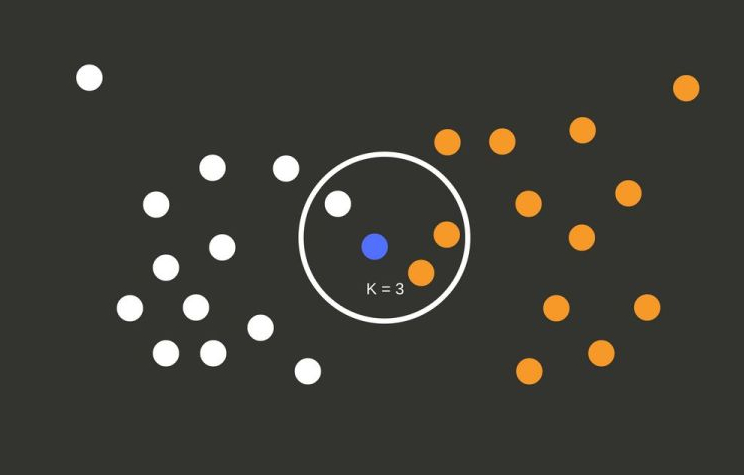
\includegraphics[width=0.5\textwidth]{images/Kn.jpg}
    \caption{Example of K-nearest neighbor. The figure shows  two different target classes orange and white circles, and one blue data point which has an unknown class. From the data points presented, we observe that the total number of the training samples  with known classes is 26. To predict the target class for the blue circle, one consider the K value as three, and calculate the similarity distance using similarity measures such as Euclidean distance \citep{K-NNALGORITHM}.}
  \label{kn}
\end{figure}

\subsection{Extremely randomized tree}

Extremely randomized tree is another tree-based ensemble method for supervised regression and classification problems. It builds an ensemble of decision trees according to the classical top-down procedure in Figure \ref{random tree}. Its differences from other tree-based ensemble methods like random forest are that the nodes are being split by choosing a threshold (cut-point) at random, and that it uses the whole training dataset rather than the bootstrap replica to grow the trees.  

As in random forest, the predictions of the trees are also combined to produce the final prediction. This is done through a process of majority voting in classification problems and arithmetic averaging in regression problems as shown in equation \ref{averageRF}. The explicit randomization of the cut-point and ensemble averaging reduces the variance even more, i.e. $\text{error}=\text{bias} - \text{variance}$ \citep{geurts2006extremely}. 







